\section{Recovery Rates}

In this section we are going to build and describe the recovery flows of the previously created stocks. The model that we are building considers all the entities relative to drug 1, which is used in the hospital. Additionally, we assume that there exists at least one antibiotic which is fully effective against any bacteria.

Both antibiotic drugs are used intensively in the hospital and we are going to indicate the rates of their usage by corresponding parameters. The rate of treatment with drug 1 is going to be named $\tau_1$. We set the initial value of 0.1 to it.

\begin{figure}[H]
  \centering
  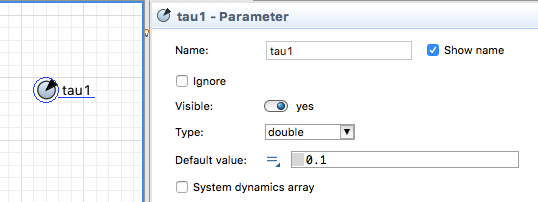
\includegraphics[height=0.3\textwidth]{img/screens/recovery/recovery1}
  \caption{Rate of treatment with drug 1}
\end{figure}

The rate of treatment with drug 2 is also very important. Without drug 2 treatment, the population of Resistant strain holder cannot remain stable. The name of the parameter is correspondingly $\tau_2$. We set its initial value to be 0.01, which is smaller than $\tau_1$.

\begin{figure}[H]
  \centering
  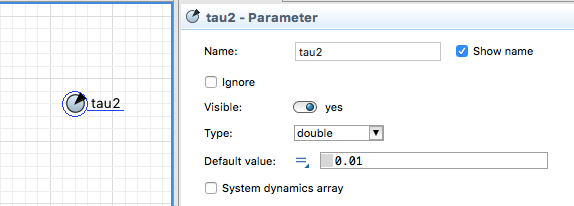
\includegraphics[height=0.3\textwidth]{img/screens/recovery/recovery2}
  \caption{Properties of the $\tau_2$ parameter}
\end{figure}

The next parameter is $\gamma$ (gamma). This variable indicates the rate of occasional recovery of any individual either from Susceptible group or from Resistant one. This kind of recoveries often happen in real life and it is truly difficult to explain the exact reason of such incidents. We set the value of this probability to be 1\%.

\begin{figure}[H]
  \centering
  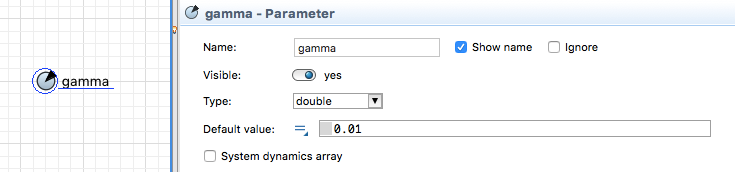
\includegraphics[height=0.25\textwidth]{img/screens/recovery/recovery4}
  \caption{Occasional treatment rate}
\end{figure}

The main parameters for the recovery flows are created now, they can be placed in the model near the previously created elements. Our next step here is to create the actual flows that will update the quantities in the stocks.

\begin{figure}[H]
  \centering
  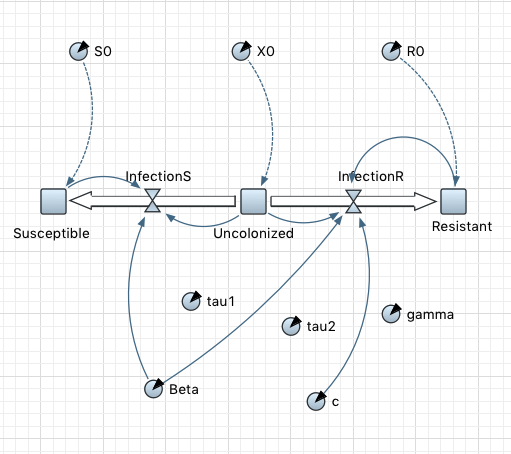
\includegraphics[height=0.5\textwidth]{img/screens/recovery/recovery3}
  \caption{The recovery rate parameters placed in the model}
\end{figure}

First of all, we know that it is more likely possible to cure the population infected with susceptible strain of the bacteria. Since the treatment with drug 1 is regular, there will always be a flow of people treated by the drug.

\begin{figure}[H]
  \centering
  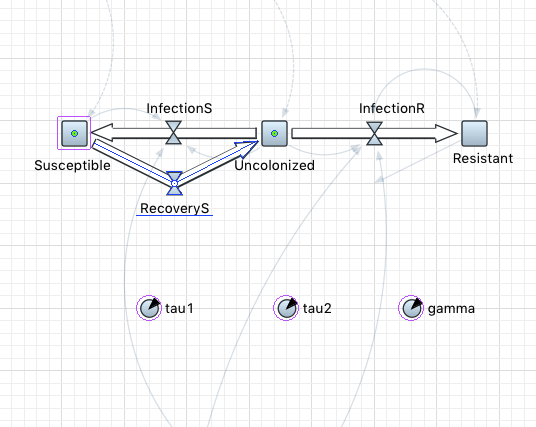
\includegraphics[height=0.5\textwidth]{img/screens/recovery/recovery6}
  \caption{The flow of Recovery from susceptible bacteria}
\end{figure}

However, the drug 1 is not the only reason. The recovery depends on other two parameters also and equals to $(\tau_1 + \tau_2 + \gamma) \cdot Susceptible$. In the properties window of the IDE, we can specify the mentioned value, which will become our differential equation.

\begin{figure}[H]
  \centering
  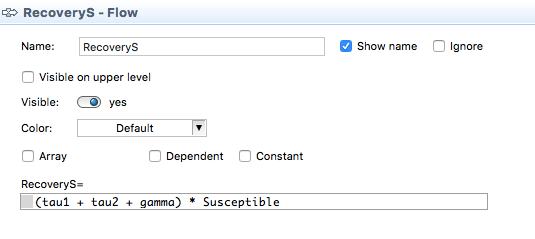
\includegraphics[height=0.3\textwidth]{img/screens/recovery/recovery5}
  \caption{The properties of RecoveryS flow}
\end{figure}

Since the used variables are already present in the model as parameters, we need to connect them to the RecoveryS flow to prevent errors. The values of the parameters will be looked up during the runtime and used to decrement the number of individuals infected by susceptible bacteria.

\begin{figure}[H]
  \centering
  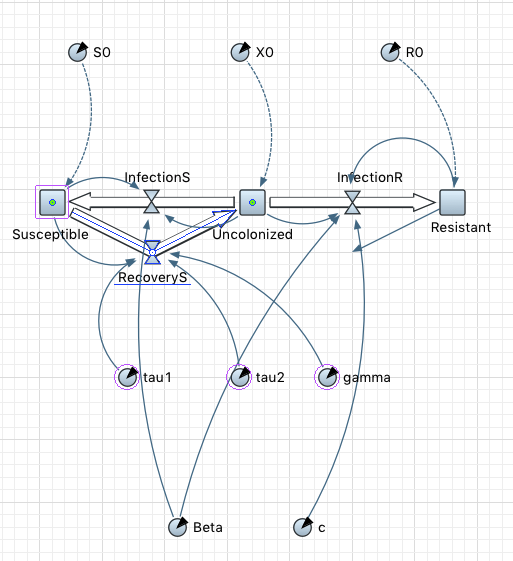
\includegraphics[height=0.6\textwidth]{img/screens/recovery/recovery7}
  \caption{Parametrization of RecoveryS}
\end{figure}

Similar to the recovery from susceptible strain, the individuals infected with resistant bacteria are also getting treated and recovered. We create the recovery flow that starts from Resistant stock and goes to the Uncolonized stock and name it RecoveryR.

\begin{figure}[H]
  \centering
  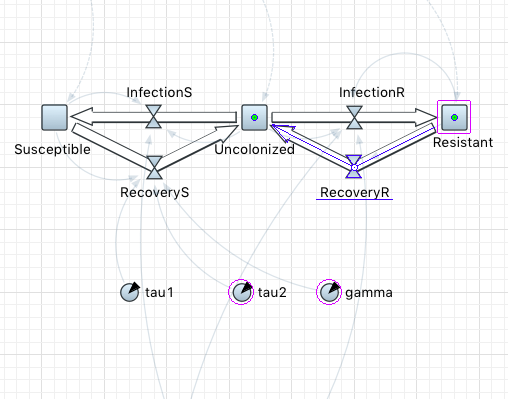
\includegraphics[height=0.5\textwidth]{img/screens/recovery/recovery8}
  \caption{The flow of Recovery from resistant bacteria}
\end{figure}

The amount of recovery from resistant strain is similar to the value of InfectionS. However, in this case the rate of recovery does not depend on $\tau_1$, the rate of treatment with drug 1. This fact is quite obvious, since the bacteria of this group are resistant to the drug 1. Therefore the recovery rate in this flow is equal to $(\tau_2 + \gamma) \cdot Resistant$.

\begin{figure}[H]
  \centering
  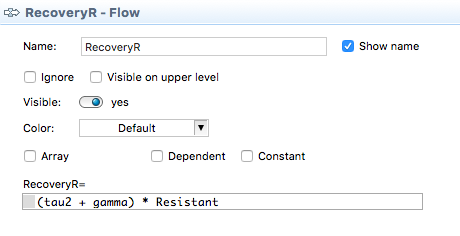
\includegraphics[height=0.3\textwidth]{img/screens/recovery/recovery10}
  \caption{The rate of recovery from resistant strain}
\end{figure}

The variables used in the specification of RecoveryR value are also already created and present in the model. To allow their usage in the expression of the flow value, we need to mark them as dependencies of the current flow. To do so, we connect them using the graphical interface.

\begin{figure}[H]
  \centering
  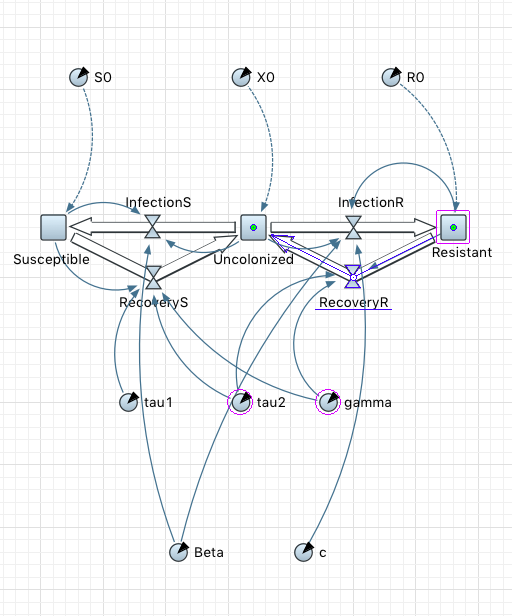
\includegraphics[height=0.6\textwidth]{img/screens/recovery/recovery9}
  \caption{Binding parameters to RecoveryR}
\end{figure}

At this point, we obtain a simulation model that has the proper circulation of the population between the observation groups. The recovery flows provide the regeneration of Uncolonized stock, making the execuion of the model much more interesting and unpredictable.

\begin{figure}[H]
  \centering
  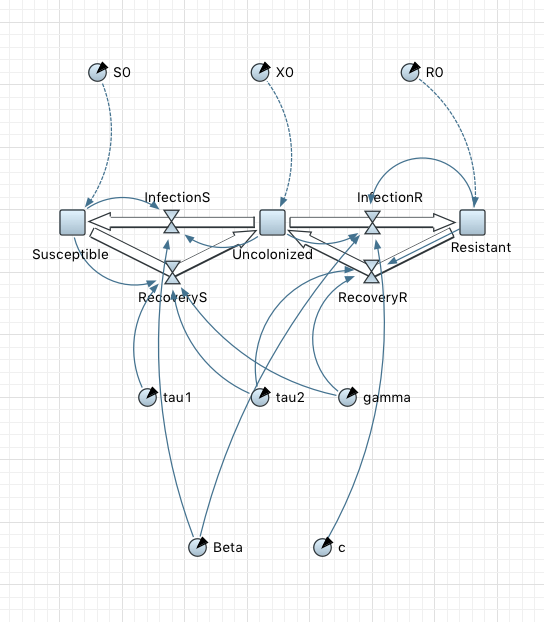
\includegraphics[height=0.6\textwidth]{img/screens/recovery/recovery11}
  \caption{The simulation model with infection and recovery}
\end{figure}